\chapter{Pseudo Random Number Generator}
\label{pseudo-random-number-generator}

% 
Há muitos anos a geração de números aleatórios é objeto de estudo da matemática. Por muito tempo não tinha um algoritmo determinístico para a geração de números que tivesse um período de repetição suficientemente longa para aplicações complexas. Em 1998, os matemáticos japoneses Matishumote e Nishimura inventaram o primeiro algoritmo em que a periocidade ( $2 ^ {19937}$ - 1) excede o número de \textbf{eletrons spin changes} desde a criação do universo. ~\cite{cristophe-diethelm} 

%
Apesar de existir o \textit{TRNG} ou \textit{True Random Number Generator}, que oferece sequências de números que são aleatórios, as mesmas não são determinísticas e isso faz com que sua utilização seja limitada, visto que em aplicações como a criptografia é necessário reproduzir a mesma sequência para a função de cifrar e de decifrar. 

%
Com isso a utilização de geradores de números pseudo aleatórios se faz necessária, porém a sequência gerada deve seguir dois critérios para que seus números possam ser considerados aleatórios:

\begin{description}
	\item [Aleatoriedade]
	O principal requisito para uma sequência ser considerada aleatória é seus números serem aleatórios. Dois critérios podem ser usados para validar uma sequência:
		\begin{description}
			\item [Distribuição uniforme]
			Os bits de uma sequência devem ter frequência aproximada, ou seja, a quantidade de 0 deve ser aproximada da quantidade de 1.
			\item [Indepêndência]
			Os números não devem ter relação entre si.
			
		\end{description}
	\item [Imprevisibilidade]
	Esse critério serve para garantir que sabendo um número da sequência, é impossível prever o número anterior ou posterior.
\end{description}

Um gerador de números pseudo-aleatórios tem como entrada uma semente \footnote{Termo para especificar um número para geração de uma sequência.} A semente normalmente é gerada de um algoritmo \textit{TRNG}. Pelo fato de serem utilizadas como entrada em algoritmos determinísticos as sementes devem ser guardadas de forma segura.

\begin{figure}[h]
	\centering
	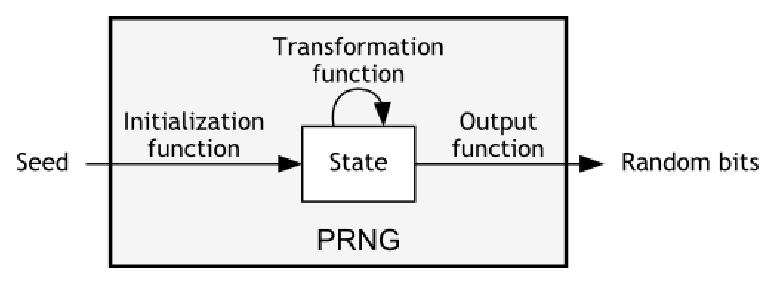
\includegraphics[scale=1]
	{figuras/prng.eps}
	\caption[Esquema de um \textit{PRNG}]{Esquema de um \textit{PRNG}\protect\footnotemark}
\end{figure}
\footnotetext{\url{http://pit-claudel.fr/clement/blog/how-random-is-pseudo-random-testing-pseudo-random-number-generators-and-measuring-randomness/}}


\section{Geradores}
\subsection{Linear Congruential Generator}

Uma técnica muito usada para geração de números pseudo-aleatórios é um algoritmo que primeiramente foi proposto por Lehmer, que é conhecido como método \textit{Linear Congruential}. \cite{william-stallings} O algoritmo gera uma sequência dependendo das entradas e a função utilizada para essa geração é:
\begin{equation}
	\label{Função para geração de números aleatórios.}
	\mathcal{X_n} = (a * X_{n - 1} + c) mod n
\end{equation}

Para cada número na sequência, essa formula é aplicada. A eficiência dessa sequência está diretamente relacionada a escolha das variáveis. A variável \textbf{m} é o módulo da equação e condição de escolha dessa variável é ser maior que 0. Para a variável \textbf{a} é o multiplicador da função e sua condição é ser maior que 0 e menor que \textbf{m}. A variável c é o incremento, sua condição é é estar entre 0 e \textbf{m}. O \textbf{$X_0$} é a semente para a sequência, será o primeiro elemento da sequência e sua condição é estar entre 0 e \textbf{m}.

A escolha dessas entradas determina a periodicidade da sequência e por consequência seu desempenho. Como exemplo de uma sequência com periodicidade 4, as entradas seriam:

\begin{table}[h]
	\centering
	\begin{tabular}{|l|l|}	
	\hline
		Variável & Valor \\ \hline
		\textbf{a} & 5 \\ \hline
		\textbf{c} & 0 \\ \hline
		\textbf{m} & 16 \\ \hline
		\textbf{$X_0$} & 1 \\ \hline
	\end{tabular}
	\caption{Parâmetros para sequência com periodicidade 4}
\end{table}

Portanto o primeiro valor da sequência é o 1, por ser a semente. O segundo valor é calculado da seguinte maneira: 

\begin{equation}
	\label{Cálculo do segundo valor}
	\mathcal{X_n} = ( 5 * 1 + 0) mod 16
\end{equation}

\begin{equation}
	\label{Resultado do segundo valor}
	\mathcal{X_n} = 5
\end{equation}

Para o terceiro valor, o cálculo é feito utilizando o resultado do anterior:

\begin{equation}
	\label{Cálculo do terceiro valor}
	\mathcal{X_n} = ( 5 * 5 + 0) mod 16
\end{equation}

\begin{equation}
	\label{Resultado do terceiro valor}
	\mathcal{X_n} = 9
\end{equation}

Finalmente para o quarto valor, também se utiliza o valor anterior em seu cálculo:

\begin{equation}
	\label{Cálculo do quarto valor}
	\mathcal{X_n} = ( 5 * 9 + 0) mod 16
\end{equation}

\begin{equation}
	\label{Resultado do quarto valor}
	\mathcal{X_n} = 13
\end{equation}

A partir do quinto valor, a sequência se repete:

\begin{equation}
	\label{Cálculo do quinto valor}
	\mathcal{X_n} = ( 5 * 13 + 0) mod 16
\end{equation}

\begin{equation}
	\label{Resultado do quinto valor}
	\mathcal{X_n} = 1
\end{equation}

Ou seja, as escolhas dos parâmetros é um passo extremamente importante para esse gerador. Um exemplo com uma periodicidade relativamente grande pode ser obtida trocando apenas o valor de \textbf{m} da resolução anterior:

\begin{table}[h]
	\centering
	\begin{tabular}{|l|l|}	
		\hline
		Variável & Valor \\ \hline
		\textbf{a} & 5 \\ \hline
		\textbf{c} & 0 \\ \hline
		\textbf{m} & 37 \\ \hline
		\textbf{$X_0$} & 1 \\ \hline
	\end{tabular}
	\caption{Parâmetros substituindo o valor de \textbf{m}}
\end{table}

A sequência gerada a partir dessas variáveis, é:

[1,5,25,14,33,17,11,18,16,6,30,2,10,13,28,29,34,22,36,32,12,23,4,20,
26,19,21,31,7,25,24,9,8,3,15]

Apesar de ter sido maior que a sequência anterior, isso não necessariamente prova sua eficiência, visto que para aplicações como a criptografia, números muito maiores seriam utilizados e sua periodicidade deve ser maior também.


\subsection{Blum Blum Shub Generator}

\section{Testes NIST SP 800-22}
